
\chapter{Software design}\label{txt.design.design}

There are many ways to implement data visualization. Still, choosing the right solution, programming language, or framework is hard, so this chapter first provides information on what this application should do. Second, it studies the existing OptaSense software and other solutions accessible from the internet. Lastly, it explains the software design decisions for implementing this data visualization.

% \section{Software design}\label{txt.design.sw}
\subsection{Usecases}\label{lab:usecases}\label{txt.design.sw.usecase}

The task is to fulfill the usage requirements, as seen in the use case figure \ref{fig:usecase}. Users need to see and view what is happening in their perimeter on their screen. For this purpose, the best data visualization is a waterfall graph, similar to a spectrogram, displayed as the main element. It should have an editable color map to adjust the sensitivity. The waterfall view should be an animated waterfall graph and ideally display real-time data on the screen, similar to the OS6 system; see Section \ref{fig:ossix}. In addition, the user should perform selection and zoom on the waterfall graph. The user should be able to edit properties of the graph, like changing the data range and choosing the channels he or she wants to see. The user should be able to export the data to a WAV file by clicking a button and then viewing and playing the audio file. There should also be a waveform display available to show the playing data.

\begin{figure}[h]
    \centering
    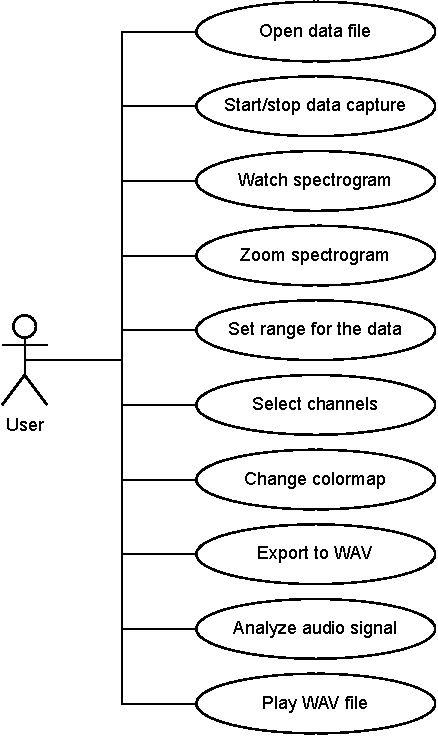
\includegraphics{pdf/usecase.drawio.pdf}
    \caption{Application usecases}
    \label{fig:usecase}
\end{figure}

\subsection{Application requirements}\label{txt.design.sw.requirements}

From the use-cases in Section \ref{lab:usecases}, it is understandable that the application should have certain features. Apart from the given use cases, there are other important requirements:

\begin{itemize}
    % \item Support for real-time data plotting - graph updates or animation; fetching the data online from the OptaSense Interrogator and displaying it in real-time
    \item Multiplatform - the application should run on any device and still support all features
    \item Data processing - subsampling data to save data throughput
    \item Plot editing and animation - changing plot properties
    \item Reading offline data - possibility to read local files or upload files into the application
    % \item 
\end{itemize}

% There is the option to create an application running on the operating system

\begin{figure}[h]
    \centering
    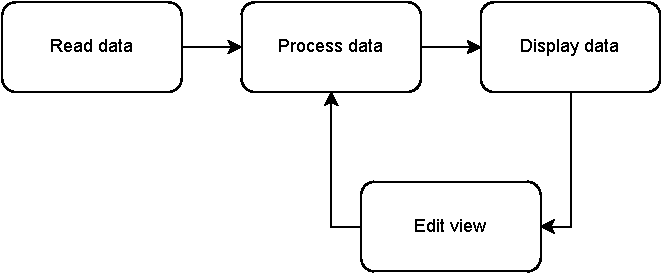
\includegraphics{pdf/simple_application.drawio.pdf}
    \caption{Data flow in the application - reading the data then processing the data and displaying it (optionally) edit the view}
    \label{fig:dataflow}
\end{figure}

It is necessary to choose the right programming tools to satisfy all features. The right way to find the right solution in programming is to \textit{divide and conquer}. This means finding all the pieces that will make the application. First, there must be an idea of what will happen with the data. Firstly, it has to be read, processed, and then displayed. The optional step is to edit the data or change the view; this data flow can be seen in Figure \ref{fig:dataflow}. 

% Multiplatform requirement removes many options - like creating a simple GUI application, as creating a multiplatform high-performance application is quite a feat and is beyond this project. So the result is making a web site and display  there is one solution either using 

From the data flow application, an overview can be made for a web application, as seen in Figure \ref{fig:app_overview}. The overview illustrates what parts the application will have. The back-end or server application will be responsible for reading HDF5 files and processing data. It will provide some interface or API for the client application to fetch\footnote{\url{https://developer.mozilla.org/en-US/docs/Web/API/Fetch\_API}} the data. On the client side, the client has to be able to create visualizations of the data and provide a user interface to change application properties.

\begin{figure}
    \centering
    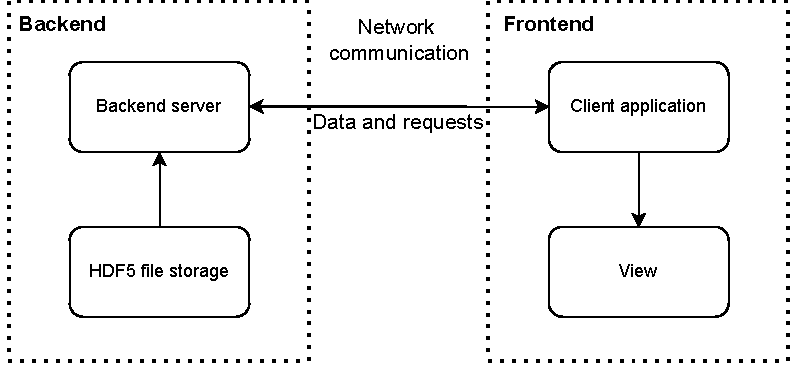
\includegraphics{pdf/appstack_general.drawio.pdf}
    \caption{Application overview. The server reads the data from the data storage and sends it to the client application, where it is shown to the user}
    \label{fig:app_overview}
\end{figure}


\section{Back-end}\label{txt.design.backend}

The purpose of the back-end part of the application is to read, process, and send the data to the client part of the application, as seen in Figure \ref{fig:app_overview}. Reading the HDF5 data is done as explained in Section \ref{txt.implementation.reading}.


\subsection{Existing REST based servers for HDF5 data access}\label{txt.design.rest}

There is a wide range of REST server implementations; HDF Group provides documentation for its RESTful API\footnote{\url{https://support.hdfgroup.org/pubs/papers/RESTful\_HDF5.pdf}}. They have prepared a few RESTful server implementations for their data format. There are many more implementations of REST servers, such as the Python Simple HTTP server. Here is a list of some possible implementations \cite{hdfrest}:

\begin{itemize}
    \item \emph{h5serv} - REST-based service to access HDF5 data written in Python (HDF5 Group).
    \item \emph{HSDS} (Highly Scalable Data Service)\footnote{\url{https://github.com/HDFGroup/hsds}} - Python implementation of the REST-based service to access HDF5 data stores. Data can be stored in the POSIX file system or object-based storage such as AWS S3. It can run in a Docker as a single machine or on a Kubernetes cluster.
    \item \emph{hdf-rest-api}\footnote{https://github.com/HDFGroup/hdf-rest-api} - is HDF5 REST API that provides CRUD support (create, read, update, and delete) for all HDF5 objects.
    \item \emph{h5grove} - Back-end service written in Python providing access to HDF5 file content.
    \item \emph{http.server} - Python implementation of a simple HTTP server. However, this is better used only for testing purposes when accessing local files.
\end{itemize}


\subsection{WebSockets}\label{txt.design.websocket}

WebSockets (or WebSocket API) enable two-way communication over \ac{tcp}. IEFT standardized it in RFC6455\footnote{https://www.rfc-editor.org/rfc/rfc6455}. All modern browsers support the WebSocket protocol.

The communication starts with an HTTP-compatible handshake, so only one socket can communicate with the server. There are also other header types available for different uses. The server responds with an HTTP Upgrade, the connection is established, and bidirectional communication can begin. Communication closes when either side decides to close the connection and starts closing the handshake. The other side responds with a \textit{Close frame} message, closing the connection. 

The protocol is frame-based, as is HTTP protocol, but simultaneously, it tries to be frame-based as little as possible. Just enough to make sure that it can use the HTTP interface for communication; otherwise, it tries to be as minimalist. The authors of the WebSocket protocol wanted it to be low-level, and as close to TCP as possible \cite{websock}. WebSockets have an implementation in the Python programming language called \verb|websockets|\footnote{https://pypi.org/project/websockets/}.

\begin{figure}[h]
    \centering
    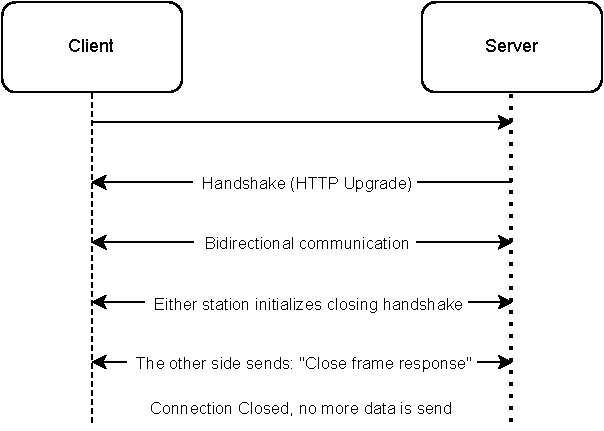
\includegraphics{pdf/websocket.drawio.pdf}
    \caption{WebSocket handshake, communication, and connection close diagram.}
    \label{fig:websocket}
\end{figure}


% \subsubsection{Processing data}\label{txt.design.datapprocessing}
% TODO???

\section{Frontend}\label{txt.design.frontend}
% \subsubsection{WebGL}\label{txt.design.frontend.webgl}
\section{Svelte}\label{txt.design.frontend.svelte}

Svelte is a component framework written in JavaScript, using a new approach to building web applications. Instead of looking for differences in virtual DOMs as React does, which is done in the browser and consumes quite a lot of resources, Svelte does everything at the compilation stage. The compilation output is a JavaScript file \verb|bundle.js|, which contains all the necessary code to run the web application or, better said, it manipulates the DOM directly. The result is a fast and reactive web page, it also saves resources, and the code can be run on small devices like handheld devices. Web development is also very enjoyable because compilation does not take long, and the changes can be visible immediately. The structure of a Svelte component consists of three parts - JavaScript code tag \verb|<script>| a style tag \verb|<style>| and other HTML elements. 

Svelte does not provide more advanced features like page routing. For this purpose, the Svelte team created SvelteKit, which is a~framework for building web applications and allows page routing. Routing is folder-based - the developer creates a folder and file structure.

\begin{verbatim}
src/routes/about/+page.svelte <=> /about
src/routes/about.svelte <=> /about
\end{verbatim}

Svelte has been changing and has become a Vite \footnote{\url{https://vitejs.dev}} plugin. Vite provides fast development experience by running a development server, in the case of Svelte - Hot Module Replacement (HMR)\footnote{\url{https://vitejs.dev/guide/features.html\#hot-module-replacement}}. This way, every change made during development can be immediately seen in the browser without reloading the page, which makes development much faster and more enjoyable. It is necessary to say that Svelte is still in development, and although it is now at version 3, it is possible that it will change in the future. 

When fetching the data from the server, it is good practice to move this functionality to a Svelte Store. From a programming point of view, a store is an object with a \verb|subscribe()| function. An example of a WebSocket implementation in Svelte can be the Svelte component library \textit{svelte-websocket-store}\footnote{\url{https://github.com/arlac77/svelte-websocket-store}}.


\subsection{Real-time capabilities}\label{txt.design.frontend.realtime}

The data bandwidth (the amount of data necessary to be sent from the server side to the client side) of the application is the biggest factor. The OptaSense Interrogator can produce quite a lot of data, but if it is saved in an HDF5 file, as it is compressed, it is quite small. As discussed in Section \ref{txt.implementation.reading}, a \qty{10}{\second} file produces around \qty{52}{MB} of data. When this data is transformed into text form, it has only \qty{420}{MB}, and when transformed into JSON, it has \qty{946}{MB} as the data are read at  \qty{10}{kSPS}\footnote{\ac{sps}}. Data will be displayed on display with standard resolution and cannot display \qty{10000}{\ac{sps}} on a small part of the display. Data processing is necessary for this purpose. 


% \subsubsection{Data processing}\label{txt.design.frontend.dataproc}

% Data processing can be done on the server or browser. As the browser will be busy redrawing waterfall visualization, it is better to preprocess data on the server side. Server-side preprocessing will also save bandwidth as the data will be significantly filtered. 

% Sending data in the form of REST requests and responses can be possible, but it is really useful only when sending a small HDF5 file as a whole, not as a stream of data, and although the h5grove backend provides the ability to read sections of the data set for  The respective bandwidth would be \qty{}{}

 % The JSON file is quite large - the original HDF5 file is only \qty{52,7}{MB} and the JSON file is \qty{946,6}{MB}. The dump text file is half the size and provides the same information, but the datasets are harder to understand, but the whole file is only half the size of the JSON file at ``only'' \qty{420}{MB}. The JSON format is much easier to read. The structure of the file is divided into three parts:


% %TODO


\subsection{Software design frontend for DAS data visualization}\label{txt.design.frontend.dataviz}

As we discussed in Section \ref{txt.design.optasense}, it is possible to create such software to display the data in real-time. The proprietary application from Optasense is a native Windows application. The requirement for this application was to be able to run on multiple platforms. The chosen platform is the Python back-end for opening files, processing the data, and sending the data to the client application using Svelte. The backend will process the data as explained in \ref{txt.design.datapprocessing}. The waterfall graph will be an HTML Canvas element that displays the data in real-time, redrawing itself as the data arrive at the browser. For ease of displaying the data in Canvas, D3.js will be used. D3 will, for example, apply a color map to the correct scale according to the data. The user interface written in Svelte will also have inputs to change the properties of the visualization so that the user can select specific channels from the data, choose subsampling effect properties, cutting the frequency range. The ability to export the data to a WAV file will also be implemented the same way as done in Section \ref{lab:hdftowav}.

\begin{figure}
    \centering
    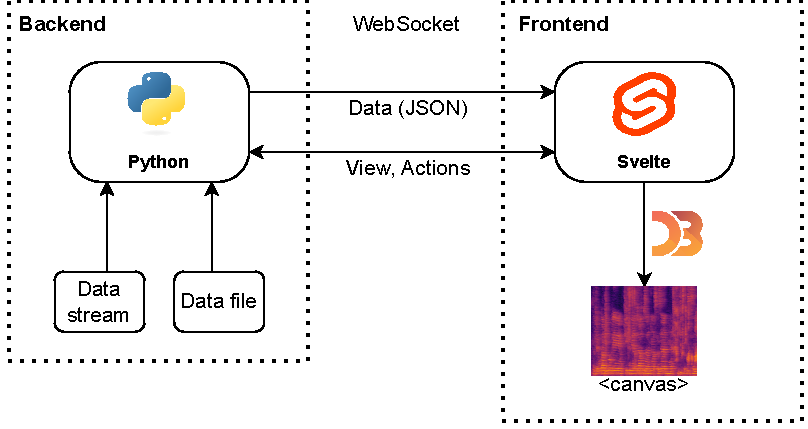
\includegraphics{obrazky/appstack.drawio.pdf}
    \caption{Application overview}
    \label{fig:app_overview}
\end{figure}







\section{HTML chart rendering}

For in-browser rendering, two main options exist using HTML canvas rendering or using \ac{svg} elements. In this section, we will discuss both their advantages over each other and their drawbacks. In general, Canvas rendering performs better than \ac{svg} rendering. This is because SVG is based on a \ac{dom} structure\footnote{text-based structure defining objects displayed on the web page. https://developer.mozilla.org/en-US/docs/Web/API/Document\_Object\_Model/Introduction}. It is more suitable for large datasets and graphics-heavy games and animations\footnote{https://www.chartjs.org/docs/latest/\#canvas-rendering}.

\subsection{HTML SVG graphics}

\ac{svg} is an XML-based markup language developed by W3C\footnote{World Wide Web Consortium www.w3.org}. It describes 2D vector graphics in XML text files. SVG supports three types of graphic objects: vector shapes, bitmap images, and text. The main advantage compared to bitmap graphics is that all the elements can be rendered at any size without losing quality. 

The description of graphics elements is the same way as the web page description written in HTML to the final web page. There are tags for different geometrical objects, for example, rectangles, ellipses, lines, and animations. Everything is defined in an XML text file which can be edited, searched, or compressed\footnote{https://developer.mozilla.org/en-US/docs/Web/SVG}.

Data visualization using \ac{svg} graphics results in smooth and sharp visualizations. It also enables interactivity with each displayed object - selecting, hovering, or zooming. Libraries for \ac{svg} manipulation manipulate text based on the data given. \ac{dthree} is a JavaScript library using HTML, SVG, and CSS to visualize data. It can bind data to the HTML DOM and then apply data-driven transformations. \ac{dthree} allows developers to create custom visualizations as it is not a charting library but a set of data visualization tools. It is also the base for other charting libraries that build on the \ac{dthree}'f framework. They include Plotly's JavaScript implementation, C3.js\footnote{https://c3js.org/} or Britecharts\footnote{https://britecharts.github.io/britecharts/}.

\subsection{Canvas graphics}

JavaScript makes drawing to the HTML \verb|<canvas>| element possible with the use of \textit{Canvas API} or \textit{WebGL API}. It can render data visualizations, game graphics, real-time video processing, and animation. WebGL can draw 2D and 3D graphics to the canvas element, but we will not be covering WebGL further. Canvas API focuses on 2D graphics. Libraries using Canvas API that make rendering to canvas easier differ on the use case - EaselJS (web game development), Konva.js (desktop and mobile applications), Chart.js, and many more. Canvas rendering depends on the resolution of the screen. 

\verb|<canvas>| tag is used for drawing graphics. You can imagine the canvas as a rectangular area with the starting point at the top left corner with coordinates (0,0) and defined width and height. By default, this area is transparent. When we want to draw to it we need to call functions from the Canvas API. They define basic shapes and primitives that can be drawn on the canvas. Rectangles and paths are the only primitive shapes that can be drawn to \verb|<canvas>| element, and more complex shapes can be drawn by combining these primitives\footnote{https://developer.mozilla.org/en-US/docs/Web/API/Canvas\_API/Tutorial/Drawing\_shapes}. Basic example of drawing to canvas can be seen in the code snippet \ref{lst:canvas.example}. Usually, the functions define certain shapes filled with color and added to the canvas. Then "clearing" functions remove what is displayed or create transparent areas. Lastly, there are "stroke" functions that create lines. 

\begin{lstlisting}[frame=single,numbers=right,caption={An example implementation of drawing to canvas.},label=lst:canvas.example,basicstyle=\ttfamily\small, keywordstyle=\color{black}\bfseries\underbar,]
function draw() {
    //First, we need a reference to canvas element
    const canvas = document.getElementById("canvas");

    //Next, we need context to draw to
    const ctx = canvas.getContext("2d");

    /**** Drawing  ****/
    
    // drawing a rectangle to canvas
    ctx.fillRect(10, 10, 100, 100);
}
\end{lstlisting}

The biggest drawback of displaying data with \verb|<canvas>| is its lack of interactivity with displayed elements and poor text rendering capabilities\footnote{https://www.w3schools.com/html/html5\_svg.asp}. The interactions are achievable but usually require "hacky" solutions like hidden canvas or invisible layers. Having more than 1000 objects rendered on screen that can be selected can also cause performance issues. 


\subsubsection{Drawing to canvas and animation}

Creating animations on canvas elements is done in two ways. Calling function \verb|setInterval()| in which a callback function is given with a time delay value in milliseconds. This was a preferred way to create animations until the implementation of the \verb|requestAnimationFrame()| method. It also takes a callback but without a time value. This is because it just tells the browser to perform an animation, so the developer doe not need to worry about managing the number of frames per second. It can perform a redraw up to the frame rate of the screen. So if the user has a \qty{60}{Hz} screen, it redraws every \qty{16.6}{ms} and respectively, if \qty{120}{Hz} screen, it redraws every \qty{8.3}{ms}. For updating at a lower FPS than the screen refresh rate, the callback is passed with a time stamp value of the request. This value can be compared with the time of the previous update, and if the delta is smaller than desired, it will not update the canvas. If the delta is bigger, it will allow the redraw.

\subsection{Heatmap visualization}\label{txt.design.frontend.heatmap}

A \textit{heatmap} is a graph depicting data values in cells in a two dimension grid. Usually, the cell shape is made of simple rectangles or squares, but any shape is possible. For example, population data can be visualized on a map or a globe. The color of each cell is a representation of the value. Choosing the right color palette; otherwise, the data can be hard to understand. We discuss color palettes in Section \ref{txt.design.frontend.colormap}. The colors used in the heatmap indicate the relative values of the data. Depending on the color palette chosen, the result can be a visualization with darker colors representing higher values and lighter colors representing lower values. Showing a color scale legend near the graph is good practice for more straightforward data interpretation.

Heatmaps are used in different scenarios as they can make data more interesting or easily understandable. They can show the relationship between two variables on two axes or display data the same way as in tables, but thanks to colors making the table more understandable. They can help to find patterns in the data or locate interest points on maps\footnote{https://chartio.com/learn/charts/heatmap-complete-guide/}.

Heatmaps are implemented in different programming languages and frameworks. Some interesting heatmap implementations are D3js \footnote{https://d3-graph-gallery.com/heatmap}, Matlab\footnote{https://www.mathworks.com/help/matlab/ref/heatmap.html}, Plotly\footnote{https://plotly.com/python/heatmaps/}.



\subsection{Colormaps}\label{txt.design.frontend.colormap}

Choosing a suitable colormap is crucial when displaying data to users. The purpose of a colormap is to understandably represent the data so that it is easy for users to understand what is displayed in front of them.  A colormap with equal steps between colors and steps in data is best perceived - called \textit{perceptually uniform colormap}. It was found that perception of color change is best understood by the human brain rather than changes in hue. 

There are four basic colormap classes based on their function:

\begin{itemize}
    \item Sequential - is used for ordering. Incremental changes in lightness and saturation of the single color, often with a single hue, for example, \textit{vidris}, \textit{plasma}, \textit{inferno}, \textit{binary}.
    \item Diverging - is used when values deviate around a middle value. It uses changes in lightness and saturation of two different colors that meet in the middle, for example, \textit{spectral}, \textit{PiYG}, \textit{BrBG}, \textit{seismic}.
    \item Cyclic - should be used for values that wrap around at endpoints. It uses two different colors that meet in the middle, beginning, and end, for example, \textit{twilight}, \textit{hsv}.
    \item Qualitative - used for displaying information without order or relationships. Miscellanneous colours, for example \textit{accent}, \textit{paired}, \textit{pastel1}.
\end{itemize}

This section was based on \cite{colormap}. The data from the DAS system is sequential, so the best type for this application is one of the sequential colormaps. D3.js has a plugin library for generating colormaps \textit{d3-scale-chromatic}\footnote{https://github.com/d3/d3-scale-chromatic}.

\begin{figure}[h!]
    \centering
    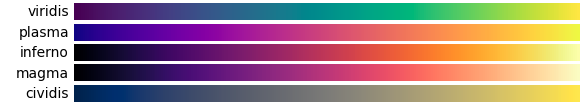
\includegraphics[width=.7\linewidth]{obrazky/sequential.png}
    \caption{Sequential colormap\cite{colormap}}
    \label{fig:colormap.seq}
\end{figure}

\begin{figure}[h!]
    \centering
    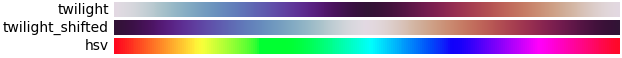
\includegraphics[width=.7\linewidth]{obrazky/cyclic.png}
    \caption{Examples of cyclic colormaps\cite{colormap}}
    \label{fig:colormap.cyc}
\end{figure}


\begin{figure}[h!]
    \centering
    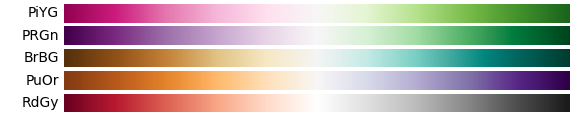
\includegraphics[width=.7\linewidth]{obrazky/diverging.png}
    \caption{Examples of diverging colormaps\cite{colormap}}
    \label{fig:colormap.div}
\end{figure}


\begin{figure}[h!]
    \centering
    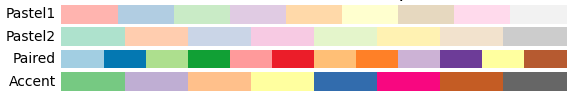
\includegraphics[width=.7\linewidth]{obrazky/qualitative.png}
    \caption{Examples of qualitative colormaps\cite{colormap}}
    \label{fig:colormap.qua}
\end{figure}



\section{Prototype}\label{txt.design.frontend.prototype}

To pitch ideas and show the design, a prototype was made. This prototype was not a final working application. The prototype was built with the Svelte framework for its high performance and fast development; see Section \ref{txt.design.frontend.svelte}. The prototype used Flowbite components\footnote{\url{https://flowbite-svelte.com/}} as they make it easy to create stylized web pages. The web page is divided into Svelte components. The main component is the waterfall graph on the left side of the screen and the control panel on the right side. Layout was done with svelte-layouts\footnote{\url{https://www.npmjs.com/package/svelte-layouts}} package. 

Uploading files into the browser using REST API was also tested. Python's \verb|http.server| was used as the back-end. When fetching files into a browser from local storage using HTTP, it is necessary to allow Cross-Origin Resource Sharing (CORS) because browsers restrict this feature for security reasons. Some resources like CSS, Web Fonts, and WebGL textures have enabled CORS. For sending HDF5 files to the browser, a special HTTP header has to be added on the server side. Without this feature, the browser would throw an error into the JavaScript console. CORS is not used for the later stages and implementation because we are not uploading whole HDF5 files.

\begin{figure}[h]
    \centering
    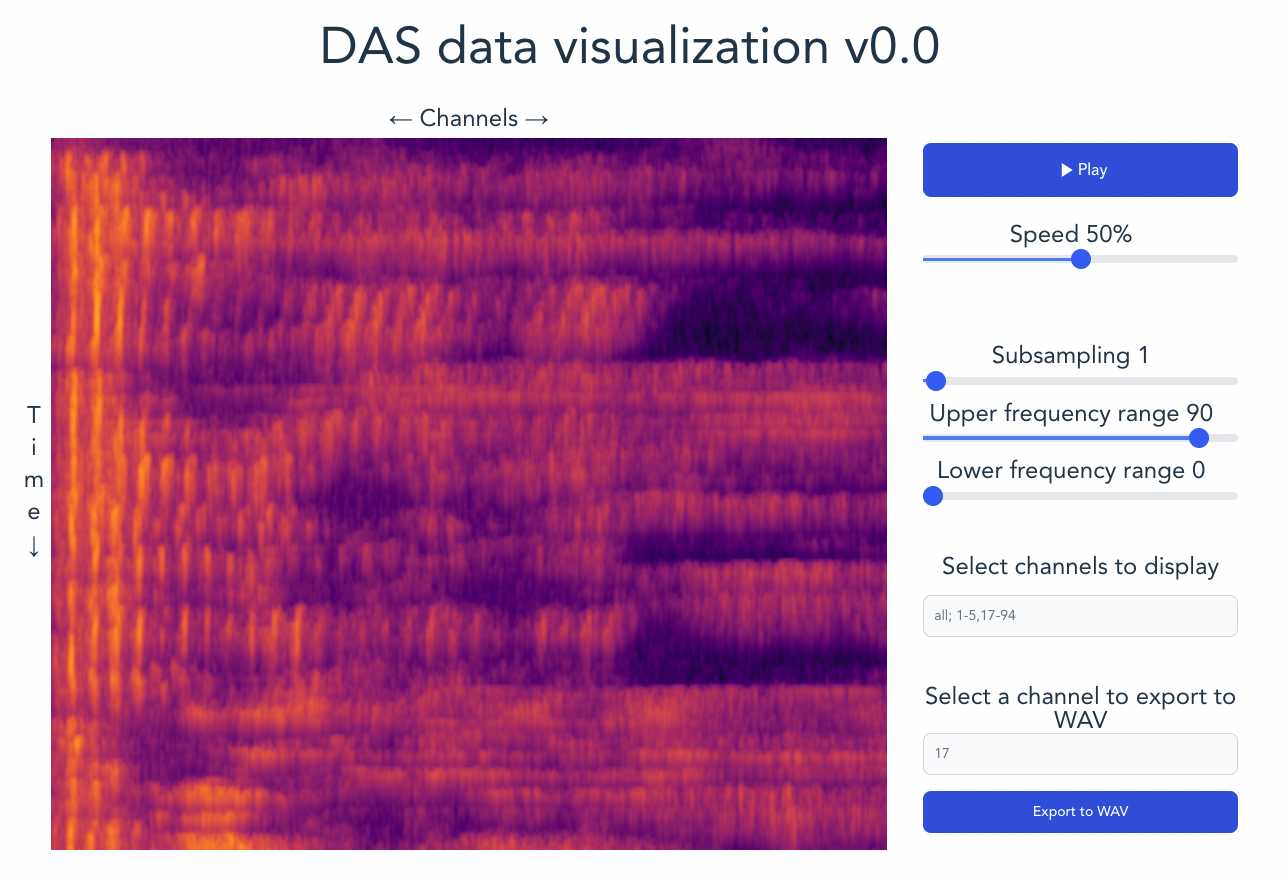
\includegraphics[width=\linewidth]{obrazky/svelte_prototype.png}
    \caption{Prototype of DAS visualization application}
    \label{fig:prototypesvelte}
\end{figure}
